\documentclass[sigconf]{acmart}

\usepackage{booktabs} % For formal tables
\usepackage{url}
\usepackage{graphicx}
\usepackage{subcaption}
\usepackage{natbib}
\usepackage{algorithm}
\usepackage{algorithmic}

\newcommand{\kai}[1]{{\bf \color{blue} [[Shukai says ``#1'']]}}
\newcommand{\heng}[1]{{\bf \color{cyan} [[Yuheng says ``#1'']]}}
\newcommand{\hao}[1]{{\bf \color{red} [[Hao says ``#1'']]}}
\newcommand{\hui}[1]{{\bf \color{purple} [[Zhenghui says ``#1'']]}}
\newcommand{\concat}{\oplus}
\newcommand{\bX}{\mathbf{X}}
\newcommand{\bx}{\mathbf{x}}
\newcommand{\bH}{\mathbf{H}}
\newcommand{\bh}{\mathbf{h}}
\newcommand{\bY}{\mathbf{Y}}
\newcommand{\by}{\mathbf{y}}
\newcommand{\bE}{\bs{E}}
\newcommand{\bA}{\bs{A}}
\newcommand{\mL}{\mathcal{L}}
% Copyright
%\setcopyright{none}
%\setcopyright{acmcopyright}
%\setcopyright{acmlicensed}
\setcopyright{rightsretained}
%\setcopyright{usgov}
%\setcopyright{usgovmixed}
%\setcopyright{cagov}
%\setcopyright{cagovmixed}


% DOI
%\acmDOI{10.475/123_4}

% ISBN
%\acmISBN{123-4567-24-567/08/06}

%Conference
\acmConference[AI]{SJTU Artificial Intelligence}{January 2018}{Shanghai, China} 
\acmYear{2018}
\copyrightyear{2018}


%\acmArticle{4}
%\acmPrice{15.00}

% These commands are optional
%\acmBooktitle{Transactions of the ACM Woodstock conference}
%\editor{Jennifer B. Sartor}
%\editor{Theo D'Hondt}
%\editor{Wolfgang De Meuter}


\begin{document}
	\title{Artificial Intelligence Course Report}
	%\titlenote{Produces the permission block, and
	%  copyright information}
	%\subtitle{Extended Abstract}
	%\subtitlenote{The full version of the author's guide is available as
	%  \texttt{acmart.pdf} document}
	
	
	\author{Zhenghui Wang}
	\affiliation{%
		\institution{Shanghai Jiao Tong University}
		\city{515021910120} 
%		\state{China} 
		\postcode{200240}
	}
	\email{felixwzh@sjtu.edu.cn}
	

	
	% The default list of authors is too long for headers.
	\renewcommand{\shortauthors}{Zhenghui Wang}
	
	
	\begin{abstract}
		In this report, we first explain the basics of several traditional and deep machine learning models. We then  
	
	\end{abstract}
	
	%
	% The code below should be generated by the tool at
	% http://dl.acm.org/ccs.cfm
	% Please copy and paste the code instead of the example below. 
	%
	\begin{CCSXML}
		<ccs2012>
		<concept>
		<concept_id>10010520.10010553.10010562</concept_id>
		<concept_desc>Computer systems organization~Embedded systems</concept_desc>
		<concept_significance>500</concept_significance>
		</concept>
		<concept>
		<concept_id>10010520.10010575.10010755</concept_id>
		<concept_desc>Computer systems organization~Redundancy</concept_desc>
		<concept_significance>300</concept_significance>
		</concept>
		<concept>
		<concept_id>10010520.10010553.10010554</concept_id>
		<concept_desc>Computer systems organization~Robotics</concept_desc>
		<concept_significance>100</concept_significance>
		</concept>
		<concept>
		<concept_id>10003033.10003083.10003095</concept_id>
		<concept_desc>Networks~Network reliability</concept_desc>
		<concept_significance>100</concept_significance>
		</concept>
		</ccs2012>  
	\end{CCSXML}
	
	%\ccsdesc[500]{Computer systems organization~Embedded systems}
	%\ccsdesc[300]{Computer systems organization~Redundancy}
	%\ccsdesc{Computer systems organization~Robotics}
	%\ccsdesc[100]{Networks~Network reliability}
	
	
	%\keywords{TODO}
	
	
	\maketitle
	
	
	\section{Introduction}
	
	
	\section{Models}
	In this section, we briefly introduce the models we leveraged in this project, from traditional machine learning models (SVM, LR, random forest) to deep models (deep neural networks and deep forest). And we conduct extensive experiments on the Human Gene Expression Dataset.
	
	
	\subsection{Logistic Regression}
	Logistic regression (LR) \cite{hosmer2013applied} is a  classical  supervised linear classifier.
	Suppose now that we are given all of the training dataset annotated with labels. We have the calculated class possibility:
	\begin{equation}
	P(Y=y_i|x_i)=\frac{e^{\omega x_i +b}}{1+\sum_i e^{\omega x_i +b}} 
	\label{lr_1}
	\end{equation}
	where $\mathbf{x}$ denotes the feature vector, $Y$ denotes label, $\omega$ denotes the regression weights and $b$ denotes the regression bias. We can determine the value of $\omega$ and $b$ using Maximum Likelihood Estimation (MLE) method with labeled training data. Assume $h_\omega(x_i)$ denoting the possibilities, the log likelihood function $L(\omega)$ is defined as:
	
	\begin{centering}
		\begin{equation}
		L(\omega)=\sum^N_i[y_i logh_\omega(x_i)+(1-y_i) log(1-h_\omega(x_i))]
		\label{lr_2}
		\end{equation}
		
	\end{centering}
	
	Various gradient-based optimize algorithm can be used to determine the value of $\omega$ and $b$. In our work, we use logistic regression in both multiple classification task and binary classification task and we compare its performance under various optimization and regularization methods.
	
	
		
	
	\subsection{Support Vector Machine}
	Support vector machine (SVM) is a supervised leanring model proposed by \citet{cortes1995support}. Its main idea is to find a hyper plane in the feature space to separate different samples into different categories, Different from other linear model like linear regression, SVM aims to maximize the \textit{margin} between two different categories' samples and the samples on the boundary are so-called \textit{support vectors}. 
	
	However, sometimes the smaples are not linear separable, then \citet{cristianini1999introduction} introduce so-called kernel trick, to project samples with finite dimensions to a high dimension or even infinite dimension space implicitly. More formally, let $\phi(\mathbf{x}_i)$ be the projected high dimension vector and $\mathbf{x}_i$ the original vector, we have:
	\begin{equation}
	\mathcal{K}(\mathbf{x}_i,\mathbf{x}_j)=<\phi(\mathbf{x}_i),\phi(\mathbf{x}_j)>=\phi(\mathbf{x}_i)^T\phi(\mathbf{x}_j)
	\end{equation}
	Some of the common kernel functions are as follows:
	\begin{enumerate}
		\item linear kernel:
		\begin{equation}
		\mathcal{K}(\mathbf{x}_i,\bx_j)=\bx_i^T\bx_j
		\end{equation}
		
		\item polynomial kernel:
		\begin{equation}
		\mathcal{K}(\bx_i,\bx_j)=(\gamma \bx_i^T\bx_j + r)^d, d>1
		\end{equation}
		
		\item RBF (Gaussian) kernel:
		\begin{equation}
		\mathcal{K}(\bx_i,\bx_j)=\exp(-\gamma ||\bx_i-\bx_j||^2),\gamma>0
		\end{equation}
		
		\item sigmoid kernel:  
		\begin{equation}
		\mathcal{K}(\bx_i,\bx_j)=\tanh(\gamma \bx_i^T\bx_j + r ), \gamma>0, r<0
		\end{equation}
	\end{enumerate}
	
	To better tailor SVM for multi-class classification problems, several methods are proposed. \citet{liu2005one} use so-called \textit{one-against-all} approach, while \citet{knerr1990single} use a more robust approach which is called \textit{one-against-one}. Briefly speaking, if we have $n$ classes, then $\frac{1}{2}n(n-1)$ classifiers are constructed. For each individual classifier, it trains data from two classes. There are also many fancy methods to construct a multi-class classifier using SVM like leveraging binary decision tree \cite{madzarov2009multi}, But we use the one-against-one approach in our experiments.


	\subsection{Random Forest}
	Random Forest \cite{breiman2001random} is one of the ensemble machine leanring models \cite{zhou2012ensemble} which could be both applied on classification and regression problems. As it is called ensemble methods, its basic components are decision trees \cite{safavian1991survey} and that the reason why it's called \textit{forest}. An illustration for random forest is shown in Figure~\ref{fig:rand-forest}. We first introduce decision tree and then random forest. 
	
	\begin{figure}[h]
	\centering
	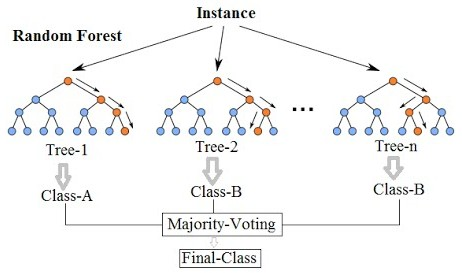
\includegraphics[width=0.8\linewidth]{../figs/rand-forest}
	\caption{An illustration for random forest.}
	\label{fig:rand-forest}
	\end{figure}
	
	A decision tree is a non-parametric supervised learning method which conduct a classification problem by make many decisions in the tree. It learns the structure of the tree by exploring all the possible plit point of every feature, and measure the quality of the split point by some \textit{purity} metrics such as information entropy $Ent(D)$ :
	
	\begin{equation}
		Ent(D)=-\sum_{k=1}^{|\mathcal{Y}|}p_k\log_2p_k
	\end{equation}
	where $D$ is the current sample set and $p_k$ is the ratio of the $k$-th class in $D$ $(k=1,2,...,\mathcal{Y})$. Obviously, $D$ is more pure if $Ent(D)$ is smaller.
	Some other purity metric includes \textit{information gain}, \textit{gain ratio} and \textit{Gini index} in CART (Classification and Regression Tree)  \cite{breiman1984classification}.
	
	Although we can use some techniques like control the minimal size of leaf node to reduce the risk of over fitting, it is still easy for decision tree to over fit. Thus, random forest (RF) is proposed \cite{breiman2001random}. It main idea is that the performance of many \textit{weak} classifiers is equal to the performance of a strong classifier. Because the diversity of many weak classifiers boost the whole model's (forest's) generalization ability. More specificly, for each split node of each tree in  RF, we do not search all the possible split points to find the \textit{best} split point. Instead, we randomly select some of the features' possible split points to find a possible best split point. This is the most important part of RF, and this is the origin of RF's diversity. More formally, suppose we have $d$ different features for each sample, we only take $k$ features into account when constructing a node. The recommend value for $k$ is $\log_2d$ \cite{breiman2001random}. If $k=1$, we randomly select only one feature. When $k=d$, the
	tree is a traditional decision tree.
	
	
	\subsection{Deep Forest}
	Deep forest (DF) is a decision tree ensemble approach with highly competitive performance to deep neural networks. It is recently proposed by \citet{zhou2017deep}. It is well known that when we talk about the term \textit{deep}, we usually mean many layers of neural networks such as the very deep convolutional neural networks' variant -- ResNet \cite{he2016deep} or the deep recurrent neural networks in temporal sequence like long short-term memory (LSTM) \cite{hochreiter1997long}. We rarely construct some kind of \textit{deep} model for traditional models, especially for those models which do not use a gradient based learning approach like random forest.
	
	However, \citet{zhou2017deep} successfully construct a multi-layer ensemble approach using traditional models -- random forest. More specificly, deep forest use so-called multi-grained sacnning (illustrated in Figure~\ref{fig:multi-grained-scanning}) to do representation learning. It is similar to the convolution operation but with a decision tree based approach. 
	\begin{figure}[h]
	\centering
	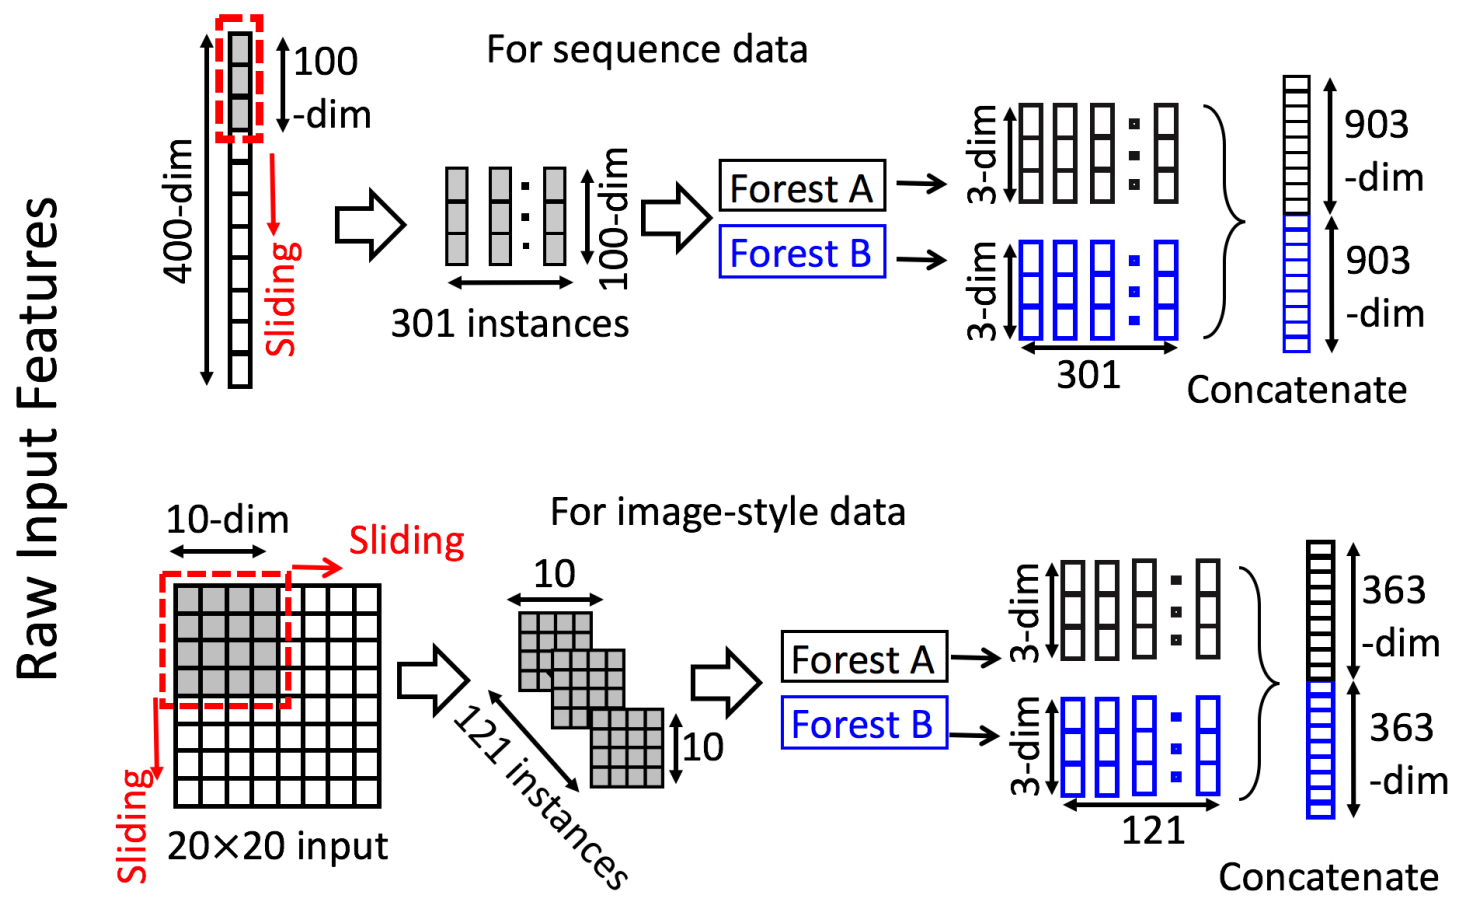
\includegraphics[width=0.8\linewidth]{../figs/multi-grained-scanning}
	\caption{ Illustration of feature re-representation using multi-grained sacnning. Suppose there are three classes, raw features are 400-dim, and sliding window is 100-dim.}
	\label{fig:multi-grained-scanning}
	\end{figure}
	
	After the multi-grained sacnning layer, a cascade forest structure is leveraged to learn better representation in a level-by-level way. Each level is an ensemble fo decision tree forest. And the \textit{diversity} is encouraged by incluing different types of forest like 2 random forests with $k=\sqrt{d}$ and 2 completely-random tree forests with $k=1$. The split is guided by the \textit{gini} value. The construction of the levels are adaptive. Each level will generate a class vector as a leared representation for next level and each level's input are the origin feature vector concatenated with early level's output class vector. For each level, we evaluate the performance with $k$-fold cross validation. If there is no significant improvement of the performance, we stop the training. The illustration for both multi-grained sacnning and cascade forest structure are shown in Figure~\ref{fig:deep-forest}, which is the whole model's pipline. 
	
	
	
\begin{figure*}[h]
\centering
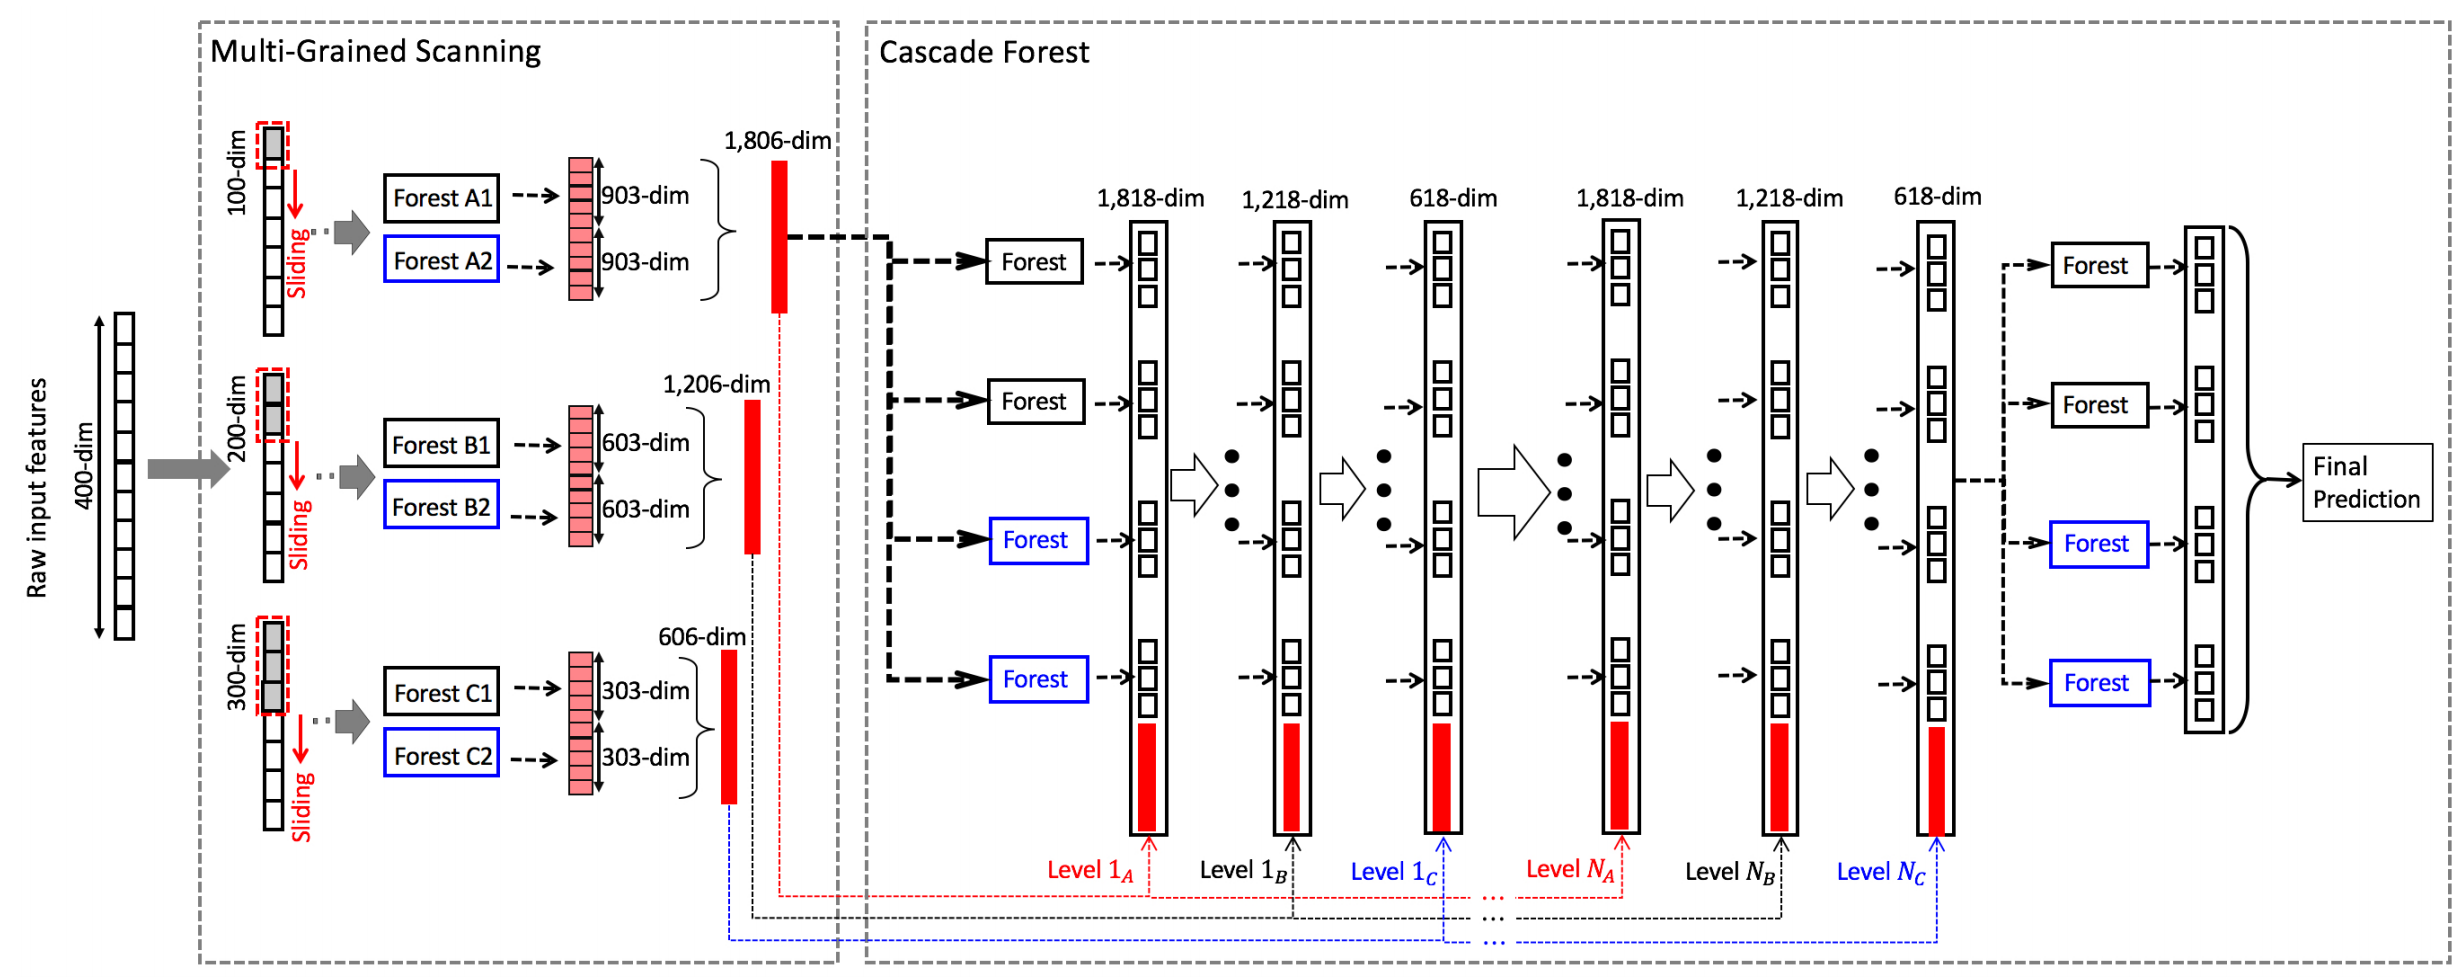
\includegraphics[width=0.9\linewidth]{../figs/deep-forest}
\caption{The overall procedure of deep forest. Suppose there are three classes to predict, raw features are 400-dim, and three sizes of sliding windows are used.}
\label{fig:deep-forest}
\end{figure*}


\subsection{Principal Components Analysis}
Principal components analysis (PCA) \cite{dunteman1989principal} aims to project the data to a lower-dimensional space in a linear way. 
And the constraint is that we want to maximize the variance of the data in low dimension. More formally, the PCA algorithm is shown in Algorithm~\ref{alg:PCA} 

\begin{algorithm}[!htb]
	\caption{Principal Components Analysis}\label{alg:PCA}
	\begin{algorithmic}[1]
		\REQUIRE
		Data matrix $X$ with size $n\times p$, where $n$ is the number of samples and $p$ is the feature dimension.
		\STATE
		Normalize the $X$ $x=x-\sum_i^N x_i$;
		\STATE
		Calculate the covariance matrix $C=\frac{X^T X}{n-1}$.
		\STATE
		diagonalize $C$, $C\gets V L V^T$, where $V$ is the matrix of eigenvectors and $L$ is diagonal matrix with eigenvalues $\lambda_i$.
		\STATE
		$i \gets 0$
		\REPEAT
		\STATE
		$i \gets i+1$
		\UNTIL{$\frac{\sum^d_i \lambda_i}{\sum^n_i \lambda_i} \ge Threshold$} 
		\STATE
		$d'\gets i$
		\STATE
		$\tilde{\mathbf{\Lambda}}\gets \text{diag}(\lambda_1,\lambda_2,...,\lambda_i)$
		\STATE
		$\tilde{\mathbf{V}}$ is the corresponding eigenvectors matrix.
		\STATE
		\textbf{output}:~~$\tilde{\mathbf{V}}\tilde{\mathbf{\Lambda}}^{1/2} \in \mathbb{R}^{m\times d'}$
	\end{algorithmic}
\end{algorithm}


\subsection{Autoencoder}
An autoencoder neural network \cite{ng2011sparse} is an unsupervised learning algorithm that applies back propagation, setting the target values to be equal to the inputs. The structure of autoencoder is show as Figure~\ref{auto_1}:
\begin{figure}[!ht]
	\centering
	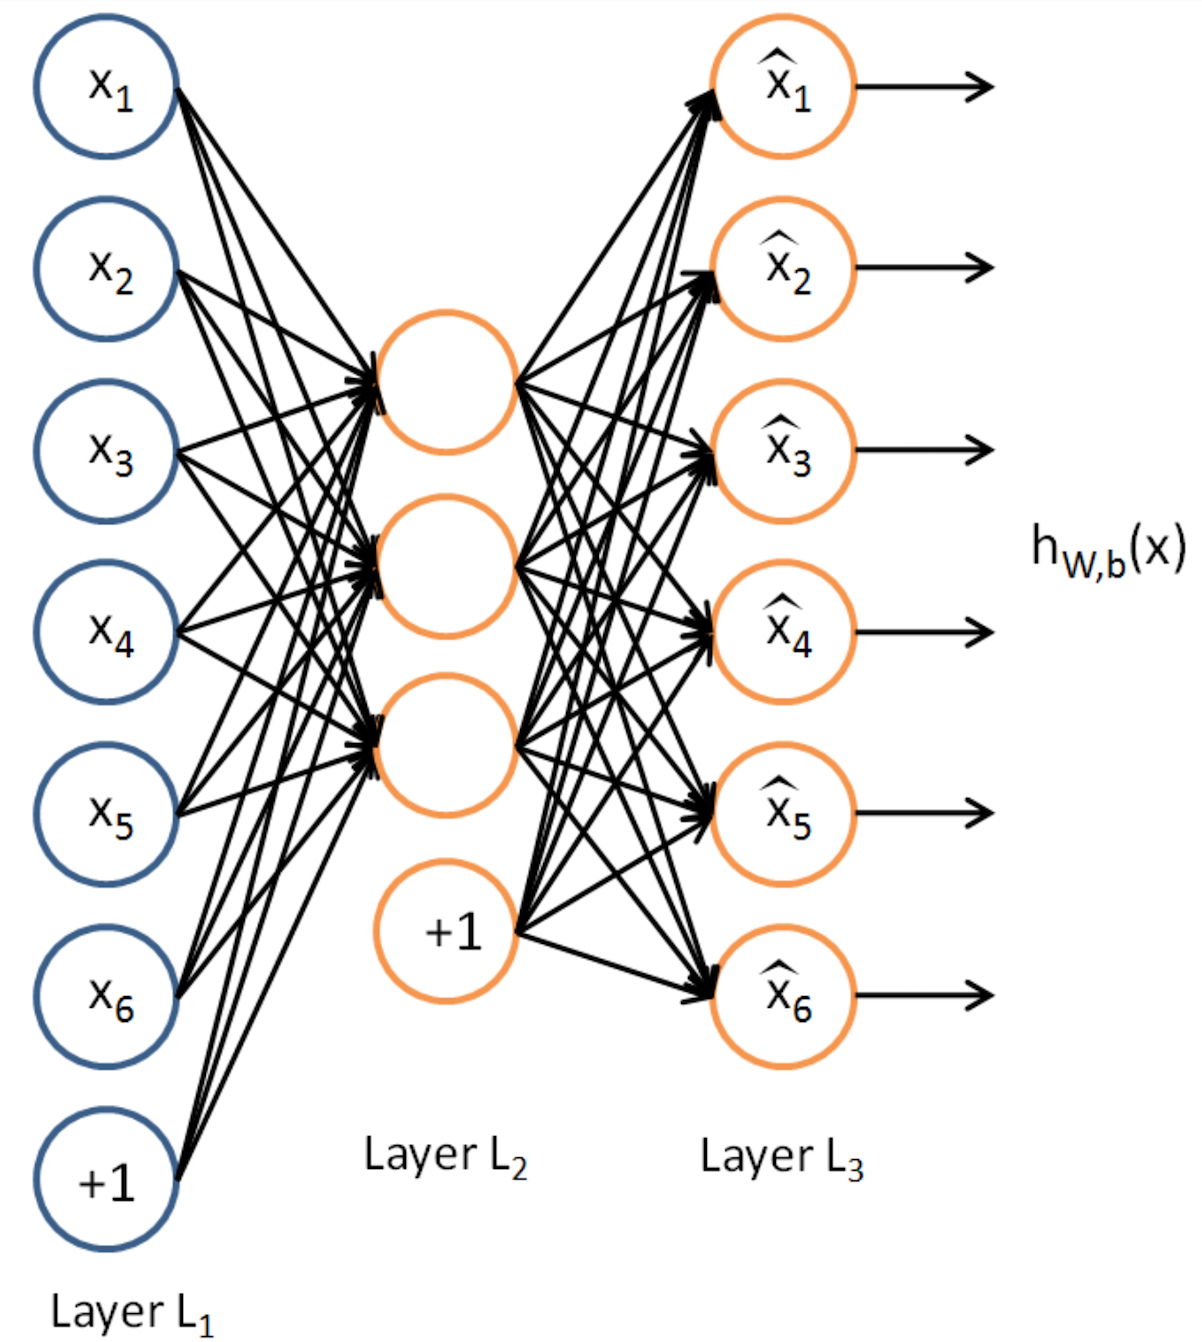
\includegraphics[width=0.3\textwidth]{../figs/auto_1.png}
	\caption{structure of autoencoder}
	\label{auto_1}
	\centering
\end{figure}

Now suppose we have  a set of unlabeled training examples $X=[x_1,x_2,x_3,\dots]$, we want $X=H_{W,b}(X)$. Then the lower-dimension output of hidden layer $L_2$ is the encoder of the raw data. This output is a nonlinear dimensionality reduction, which may overcome the weakness of PCA that it is only a linear dimensionality reduction method.


\subsection{Deep Neural Network}
Deep learning \cite{Deeplearning} has been shown as a successful machine learning method for a variety of tasks. In our work, we use a deep neural network with fully-connected multilayer structure both on PCA-processed data and on raw data with \textbf{greedy layer-wise pre training}. Besides, we add L2 regularization in each fully-connected layer to avoid overfitting and control the model complexity.
\subsubsection{network structure} Since the features do not have any locality or direct relationship, we don¡¯t use convolutions.\\

\begin{itemize}
	\item \textbf{NN on PCA-processed data}\\
	In this model, firstly we use PCA-processed data (500-dimension) as our network input. Then we add hidden layer1(256-dimension), hidden layer2(512-dimension), hidden layer3(256-dimension), finally a output layer.  The structure is shown as Figure~\ref{nn_1} network \romannumeral1. 
	For weight initialization, we initialize each neurons weight vector as a random vector sampled from a multi-dimensional gaussian. For bias initialization, we set the bias vectors all to $0$. We initialize our weight with the consideration that the size of our network is limited and it can be trained easily according to the network \romannumeral2.
	
	\item \textbf{NN on raw data}\\
	In this model, we use the raw data as the network inputs. Then we add hidden layer1(8192-dimension), hidden layer2(512-dimension), hidden layer3(128-dimension), finally a output layer.  The structure is shown as Figure~\ref{nn_1} network \romannumeral2. Since we did not use the low-dimension data, the training become much harder according to out experiment. So the network initialization is very import. We use greedy layer-wise pre training , which is a pre-train method based on the idea of autoencoder, to initialize the network. 
\end{itemize}

\begin{figure}[!ht]
	\centering
	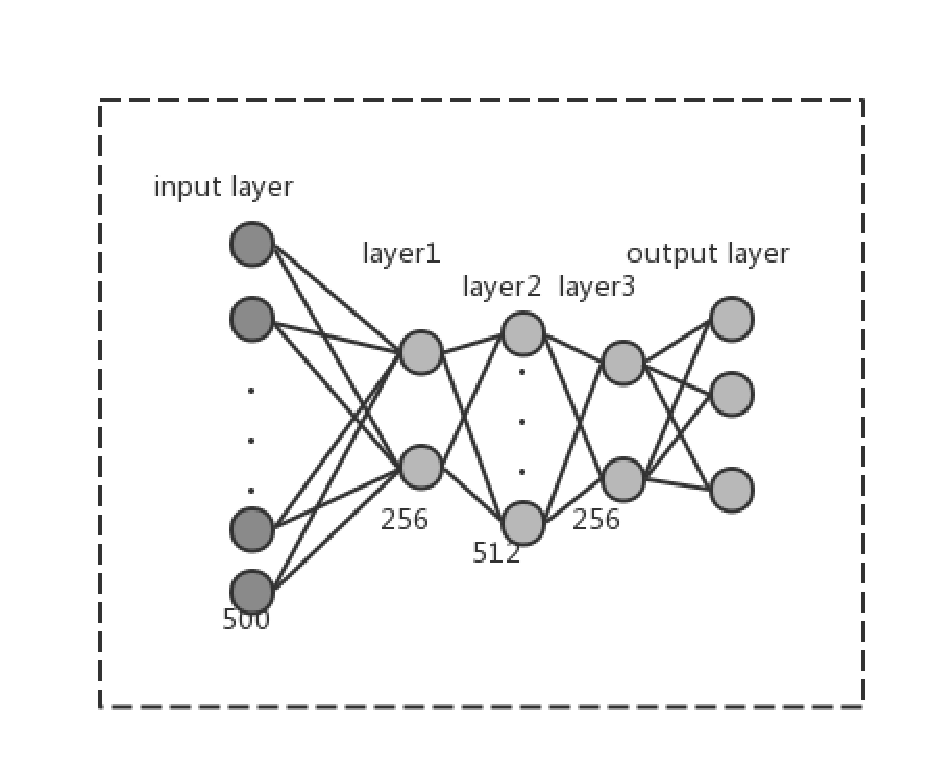
\includegraphics[width=0.24\textwidth]{../figs/nn_pca.pdf}
	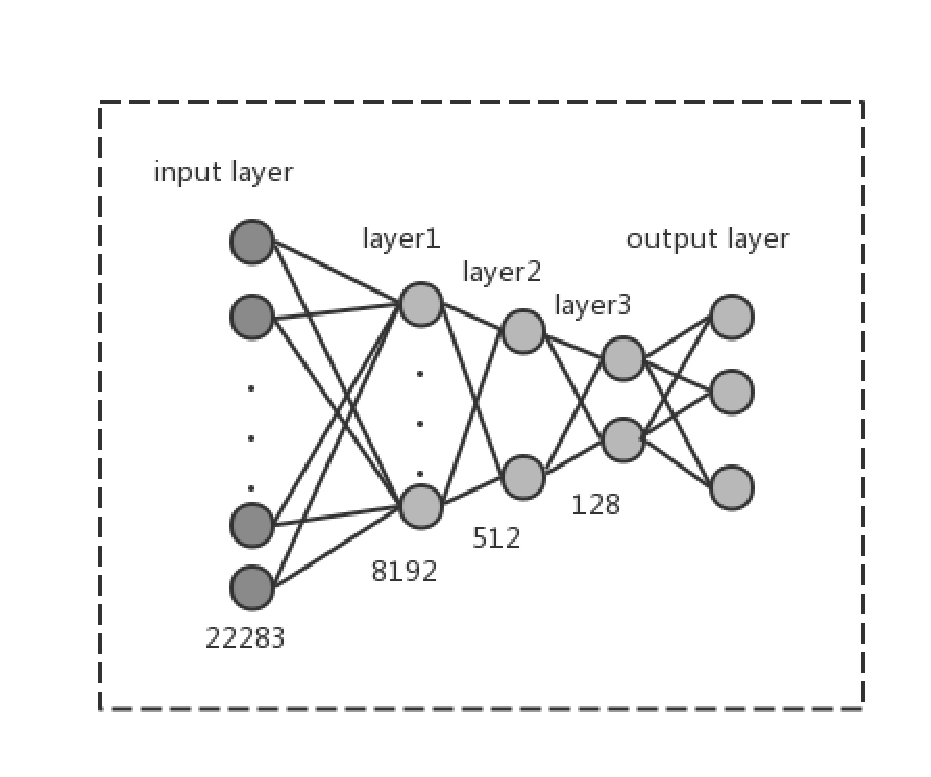
\includegraphics[width=0.24\textwidth]{../figs/nn_raw.pdf}
	\caption{a.network \romannumeral1;  b, network \romannumeral2}
	\label{nn_1}
	\centering
\end{figure}

\subsubsection{Regularization}
We use L2 regularization in each fullt-connected layer.It can be implemented by penalizing the squared magnitude of all parameters directly in the objective. For every weight $w$ in the network, we add the term $1/2¦Ëw$ to the objective, where ¦Ë is the regularization strength. This can help control the capacity of neural networks to prevent overfitting.

Furthermore, we employ Dropout \cite{Dropout} to prevent overfit- ting. While training, dropout is implemented by only keep- ing a neuron active with some probability p, or setting it to zero otherwise.

\subsubsection{Pre-train}
In network \romannumeral2, the training get very hard because of the high dimension of the network. We use \textbf{greedy layer-wise pre training} to pre-train. It will determine the initial weights of each layer layer by layer with the idea of autoencoder. Since each layer has been local optimal solution, the training get much easier .

More specifically, to determine weights of first hidden layer, we use the network shown as Figure~\ref{auto_1}. Once we get $X=h_{\omega,b}(X)$, it means the hidden layer can encode the input properly, at the same time it can pass these extracted feature to the following layer. Seemingly, when we initialize the second hidden layer, we use the output of the first hidden layer as the input of network in Figure~\ref{auto_1}. Thus we can determine all the weights. The process is show as Figure~\ref{pretrain_1}. The network \romannumeral4  in  Figure~\ref{pretrain_1} is we want, so to determine the 3 layers weights, we use network \romannumeral1-network \romannumeral3 (which are same as  Figure~\ref{auto_1}) to train them.

\begin{figure}[]
	\centering
	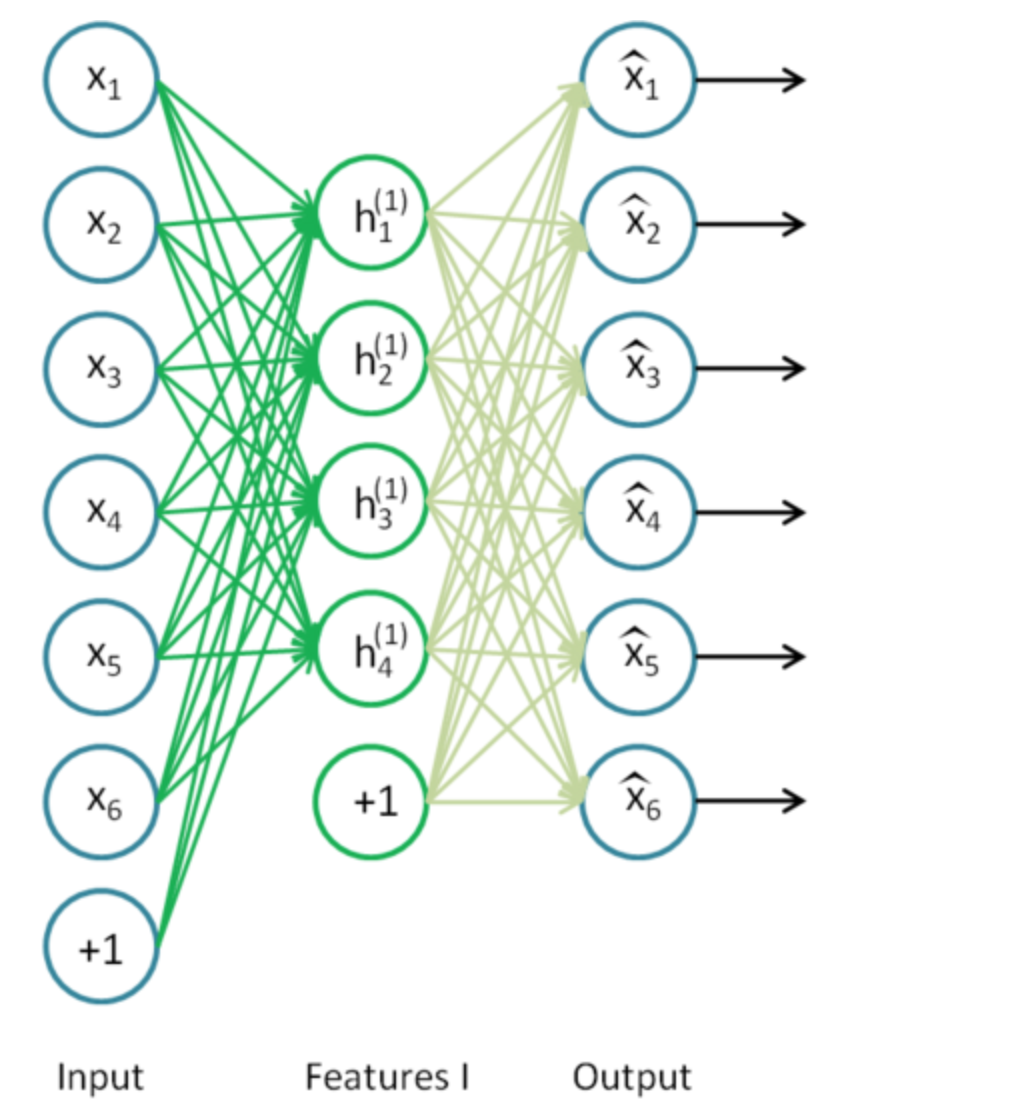
\includegraphics[width=0.2\textwidth]{../figs/pretrain1.png}
	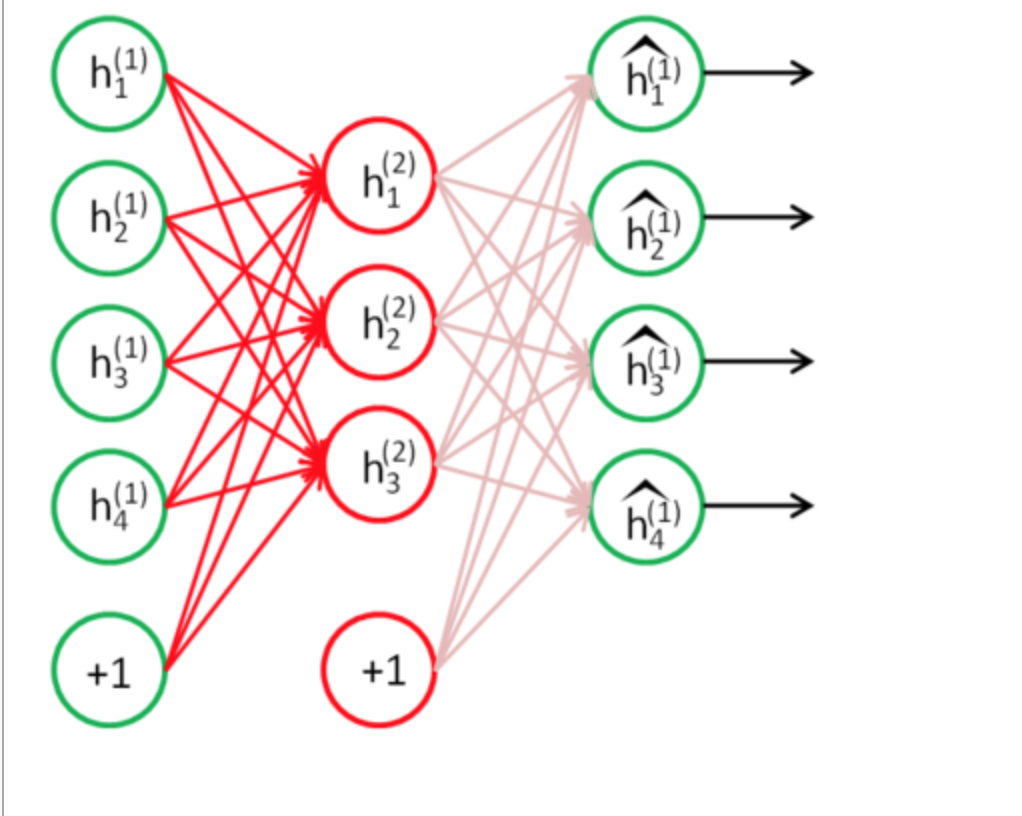
\includegraphics[width=0.2\textwidth]{../figs/pretrain2.png}
	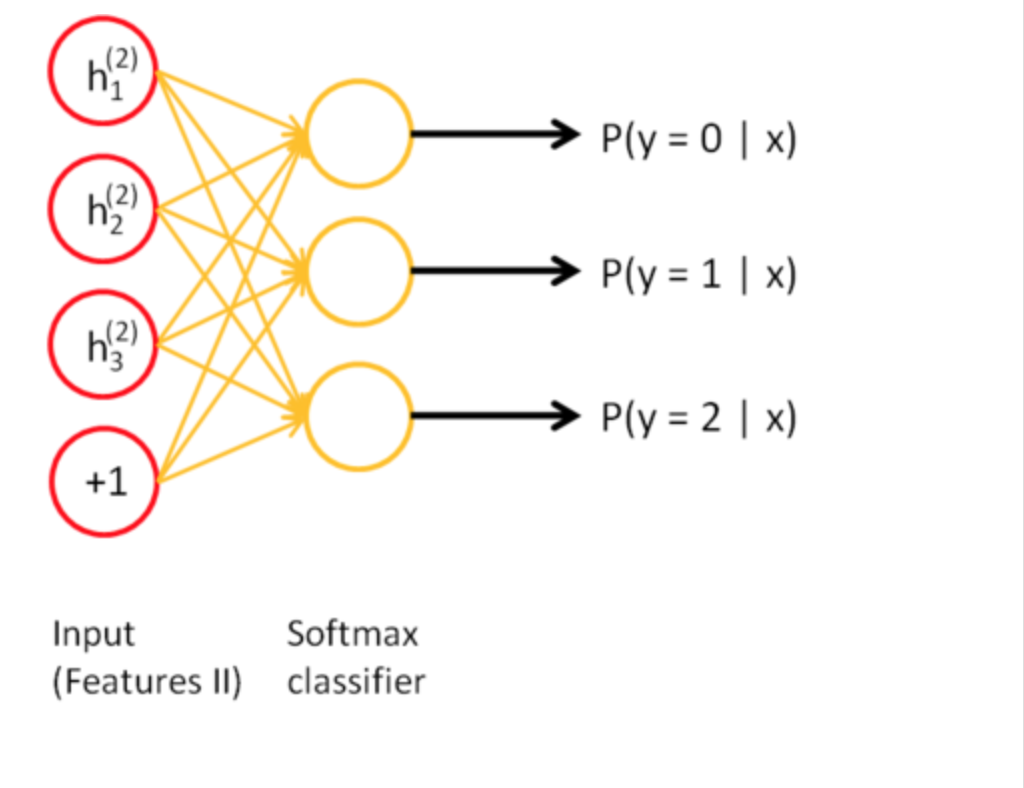
\includegraphics[width=0.2\textwidth]{../figs/pretrain3.png}
	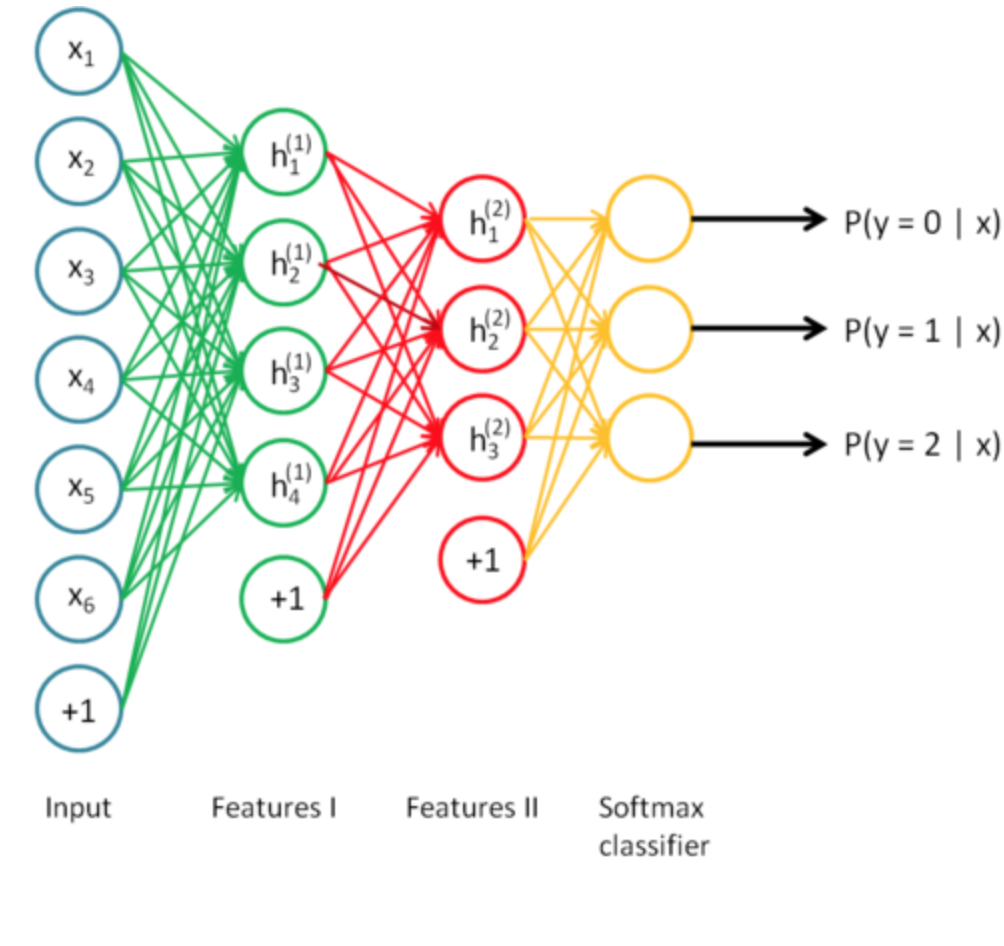
\includegraphics[width=0.2\textwidth]{../figs/pretrain4.png}
	\caption{a.network \romannumeral1;  b, network \romannumeral2; c, network \romannumeral3; d, network \romannumeral4 (From left to right and top to down). }
	\label{pretrain_1}
	\centering
\end{figure}

	
	\section{Experiment}
	In this section, we describe the experiment settings, which includes the data processing, parameter settings for each model and other details.
	
	\subsection{Label Selection}
	Since there many labels in the dataset, we have to choose some of them to be the classification objective. The first label we choose is \textit{MaterialType}, for every sample has this label. We also choose \textit{Sex} (female \& male) for it is also very important label though many of the samples' Sex label is empty. The third and fourth labels we choose are \textit{DiseaseState} and \textit{BioSourceType}, and the statistics of this two labels are show in Figure~\ref{fig:Stat_DiseaseState} and \ref{fig:Stat_BioSourceType}. We can see that both labels are long-tailed distributed, so we only choose those labels which has more than 50 samples. 
	
	\begin{figure}[h]
	\centering
	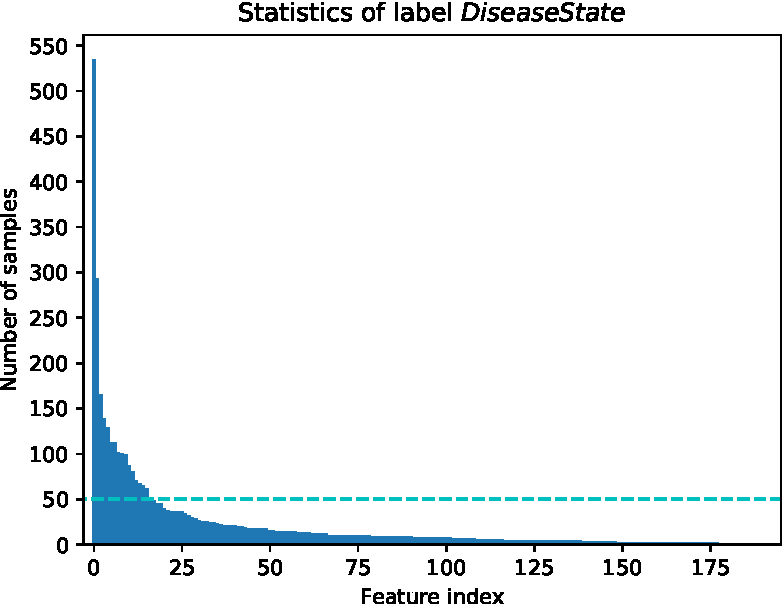
\includegraphics[width=0.8\linewidth]{../figs/Stat_DiseaseState}
	\caption{Statistics of label \textit{DiseaseState}}
	\label{fig:Stat_DiseaseState}
	\end{figure}
	
	\begin{figure}[h]
	\centering
	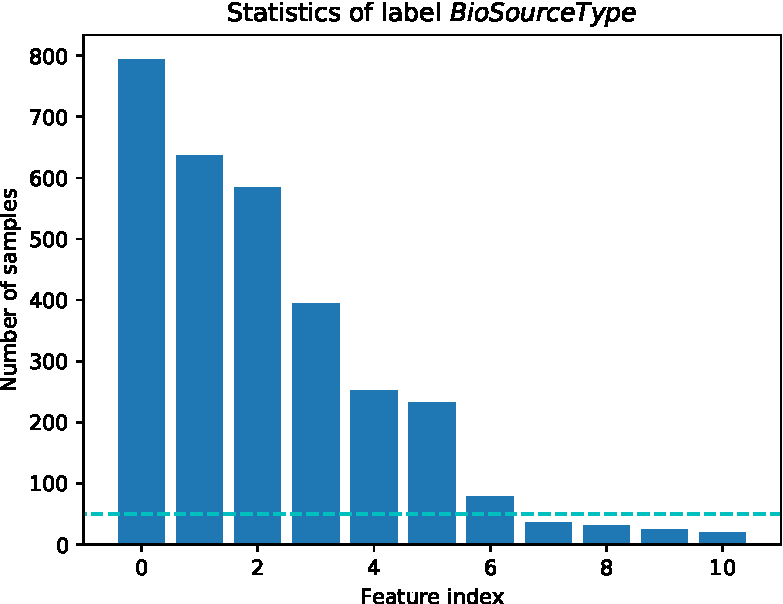
\includegraphics[width=0.8\linewidth]{../figs/Stat_BioSourceType}
	\caption{Statistics of label \textit{BioSourceType}}
	\label{fig:Stat_BioSourceType}
	\end{figure}
	
	
	we choose 4 of the labels as our classification objective. The statistics of the 4 labels are shown in Tabel~\ref{tab:label}
	\begin{table}[tbp]
		\centering
		\begin{tabular}{l|cc}
			\toprule
			{Label Type} & \# Category & \# Samples \\
			\midrule
			{\textit{MaterialType}}& 2 & 5896 \\
			{\textit{Sex}}		& 2 & 1536     \\
			{\textit{DiseaseState}}& 16 & 3493 \\
			{\textit{BioSourceType}}& 7 & 2293 \\
			\bottomrule	
		\end{tabular}
		\caption{ Statistics of the 4 labels used in our experiments. }
		\label{tab:label}
	\end{table}
	
	
	Besides, we visualize the given data with selected labels into 2-D figure using PCA method, which is shown in Figure~\ref{distribution_1}. By observation, data with Bio-7 label, Material-2 label and Disease-16 have clear boundary while it is very hard to identify the data with Sex-2 label in 2-D space.

	\begin{figure}[]
		\centering
		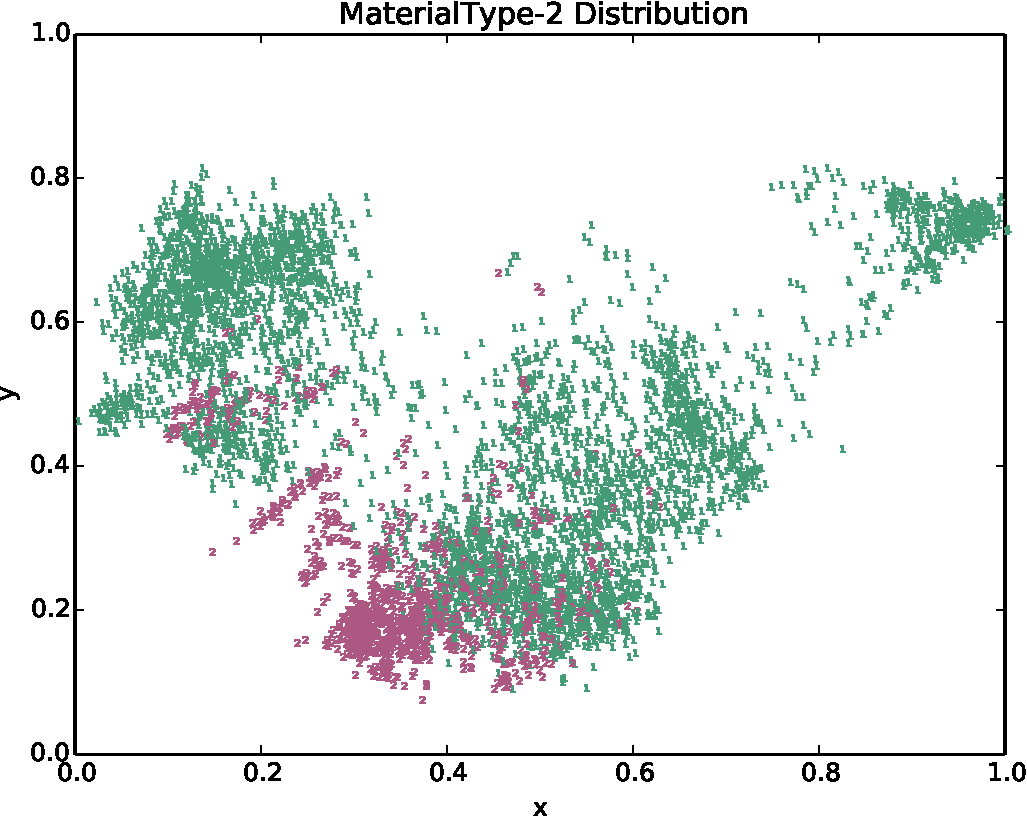
\includegraphics[width=0.2\textwidth]{../figs/Material-2.pdf}
		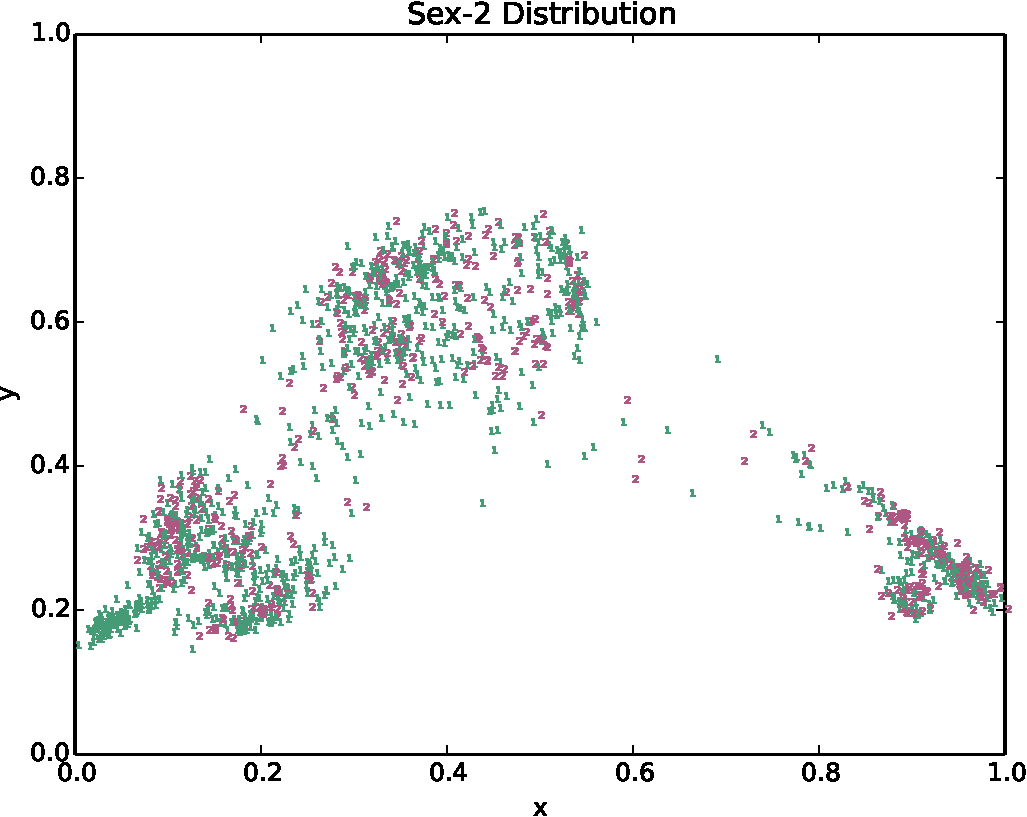
\includegraphics[width=0.2\textwidth]{../figs/Sex-2.pdf}
		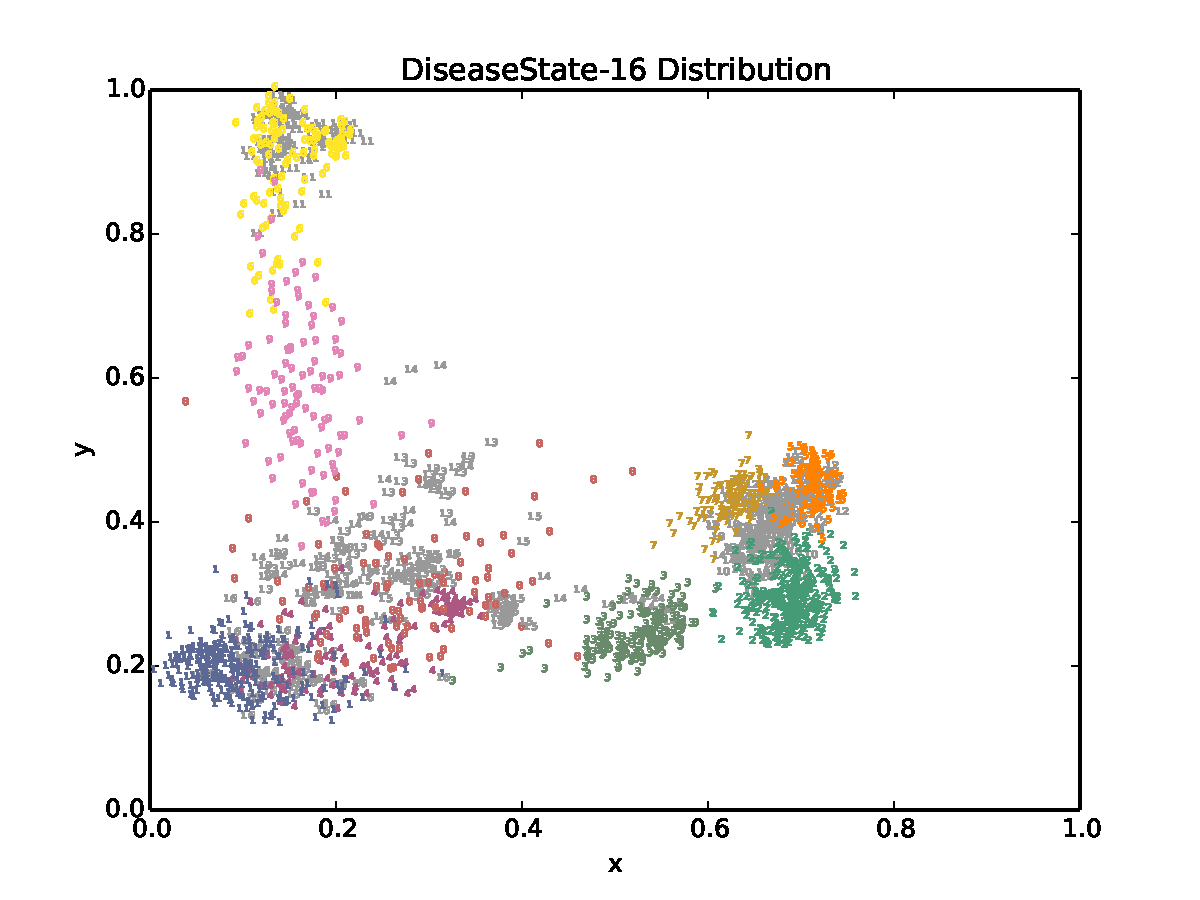
\includegraphics[width=0.2\textwidth]{../figs/Disease-16.pdf}
		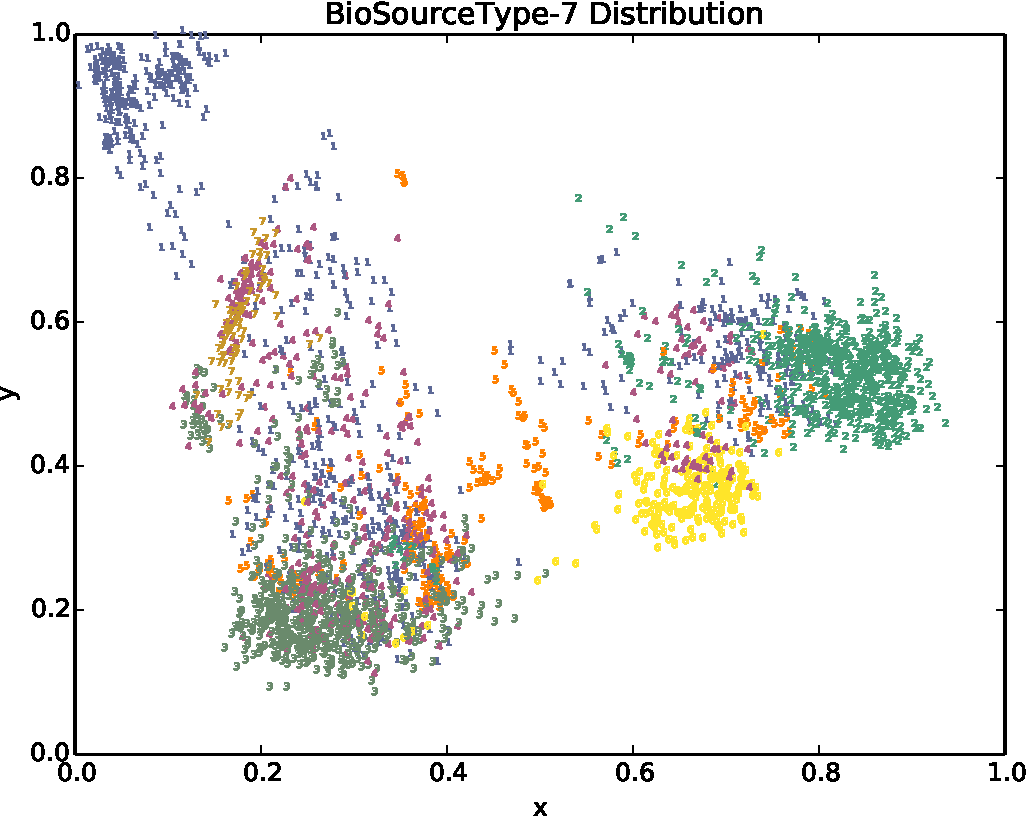
\includegraphics[width=0.2\textwidth]{../figs/Bio-7.pdf}
		\caption{a.Material-2 Distribution;  b, Sex-2 Distribution2; c, Disease-16 Distribution; d,Bio-7 Distribution (From top to down). }
		\label{distribution_1}
		\centering
	\end{figure}
	
	\subsection{Experiment Details}
	\subsubsection{Cross Validation}
	In order to get a promising results, all the experiments are conducted with the same 5-fold separation for cross validation.  
	
	\subsubsection{Problem formulation}
	For label \textit{MaterialType} and \textit{Sex}, since there are only two categories, we conduct binary classification. For label \textit{DiseaseState} and \textit{BioSourceType}, we conduct multi-class classification.
	
	\subsubsection{Evaluation Metric}
	As shown in \textit{DiseaseState} and \textit{BioSourceType}, the distribution of different categories is not balanced, so simply use accuracy is not a realistic. Instead, we tend to choose $F_1$-score as our evaluation metric, because it take both precision $P$ and recall $R$ into account. We have:
	\begin{equation}
	P=\frac{TP}{TP+FP} \nonumber
	\end{equation}
	\begin{equation}
	R=\frac{TP}{TP+FN} \nonumber
	\end{equation}
	where TP is True Positive, FP is False Positive and FN is False Negative. And $F_1$ is defined as the harmonic mean of $P$ and
	$R$ : 
	\begin{equation}
	F_1=2\cdot\frac{P\cdot R}{P+R} \nonumber
	\end{equation}
	When there are multiple classes, we use so-called Micro $F_1$-score as the evaluation metric.
	
	\subsubsection{Implementation}
	Our deep neural networks is implemented based on \textit{Keras} \cite{chollet2015keras}. The deep forest model is based on the release by \citet{zhou2017deep}, and rest of the model are implemented based on scikit-learn \cite{scikit-learn}.
	
	\subsection{Dimensionality Reduction}
	The original data is a large $p$ small $n$ problem. So we have to do some dimensionality reduction and we employ PCA to do so. We reduced the original data (22283 dimension) to different dimensions (100,200,400,500,1000,1200,2000,3400) and the ratio of reserved variance are shown in Tabel~\ref{tab:PCA}.
	
	\begin{table}[tbp]
		\centering
		\begin{tabular}{l|c}
			\toprule
			Dimension & Reserved Variance (\%) \\
			\midrule
			100 & 80.64 \\
			200 & 85.43 \\
			400 & 89.33 \\
			500 & 90.47 \\
			1000 & 93.78 \\
			1200 & 94.65 \\
			2000 & 96.99 \\
			3400 & 99.00 \\			
			\bottomrule	
		\end{tabular}
		\caption{ Reserved Variance (\%) of different reduced dimension. }
		\label{tab:PCA}
	\end{table}
	
	To determine the suitable dimension considering both feature representation ability and computation complexity, we evaluate these different dimension data in all the 4 tasks using a SVM classifier with linear kernel. The result is shown in Figure~\ref{fig:PCA_Dimension} and we find that when dimension is greater than 500, the performance of SVM in all the 4 tasks will meet a bottle neck. So we choose to reduce the original data into 500 dimensions and this 500 dimensions data are used for experiments of SVM, LR, RF and DF.
	
\begin{figure}[h]
\centering
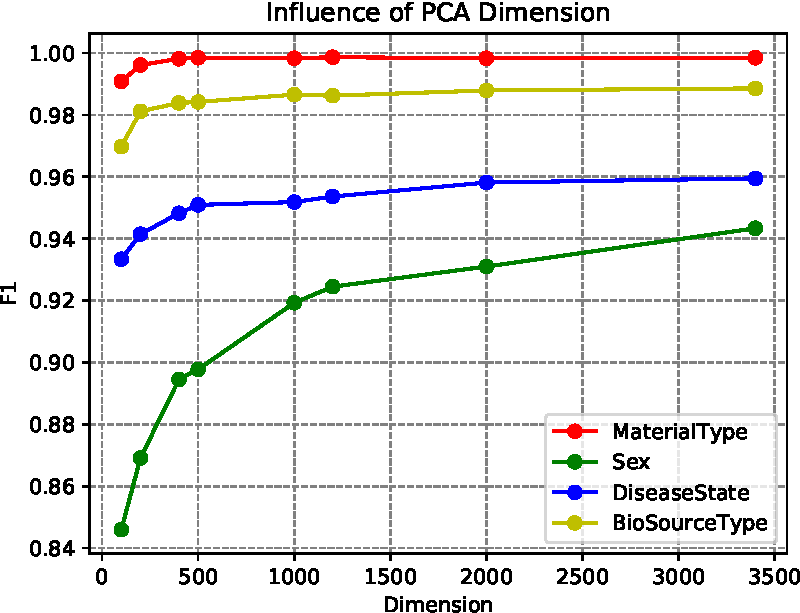
\includegraphics[width=0.8\linewidth]{../figs/PCA_Dimension}
\caption{The performance of SVM in 4 tasks with different data reduced dimensions.}
\label{fig:PCA_Dimension}
\end{figure}
	
\section{Results \& Analysis}
The experiment results and analysis will be presented in this section.


\subsection{Logistic Regression} 
We apply logistic regression to four task. Besides, we try different regularization method and solver  with different regularization strength C . We want to choose the best parameter settings and compare the preformence of different regularization method and solver. The result with the change of C is shown as Figure~\ref{lr_result1}. It can be seen that the performance of LR did not vary too much with the change of C, which may mean the data distribution is ideal and the  regularization of this model is not necessary.

\begin{figure}[!ht]
	\centering
	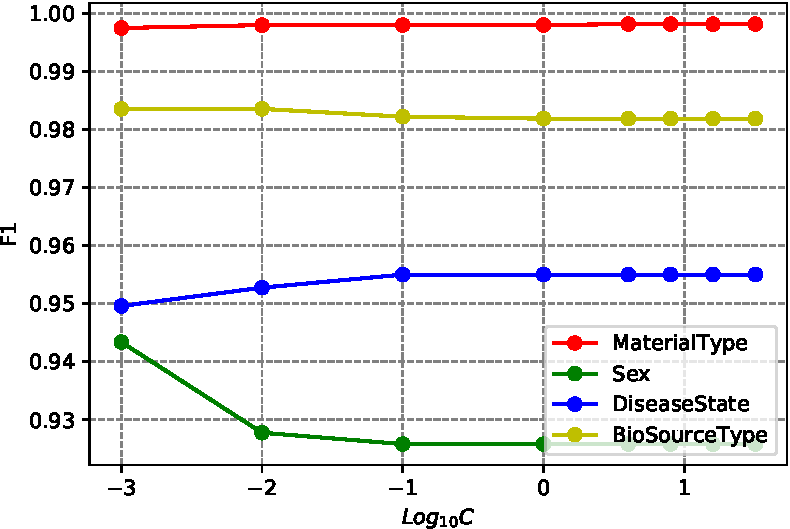
\includegraphics[width=0.4\textwidth]{../figs/LR_C.pdf}
	\caption{The performance of LR in 4 tasks with different regularization strength.}
	\label{lr_result1}
	\centering
\end{figure}

And the best results on 4 tasks with selected parameters is shown in Table~\ref{lr_result2}.

\begin{table}[tbp]
	\centering
	\begin{tabular}{l|cccc}
		\toprule
		{Label Type} & $F_1 (\%)$ & C &solver &penalty \\
		\midrule
		{\textit{MaterialType}}&99.86 & 4 &lbfgs & l2\\
		{\textit{Sex}}		& 94.96 & 0.001    &sag & l2 \\
		{\textit{DiseaseState}}& 95.72 & 0.001 &lbfgs & l2\\
		{\textit{BioSourceType}}& 98.42 & 0.01 &lbfgs & l2\\
		\bottomrule	
	\end{tabular}
	
	\caption{Best results and parameter settings for Logistic Regression. }
	\label{lr_result2}
\end{table}

\subsection{SVM}
We try different kernels (polynomial, RBF and sigmoid) with different $C$ and $\gamma$ for SVM model, because we want to find not only the best parameter settings but also how the parameters influence the model performance. 

We first evaluate the influence of $\gamma$ in polynomial, RBF and sigmoid kernel and the results are shown in Figure~\ref{fig:gamma_poly}, \ref{fig:gamma_rbf} and \ref{fig:gamma_sigmoid}. We can find that polynomial kernel is more stable to $\gamma$, while RBF kernel and sigmoid kernel are much more sensitive to $\gamma$. This also indicates that the choice of kernel and parameter tuning is vary important in SVM and some kernels (polynomial kernel here) are more robust in some conditions.

\begin{figure}[h]
\centering
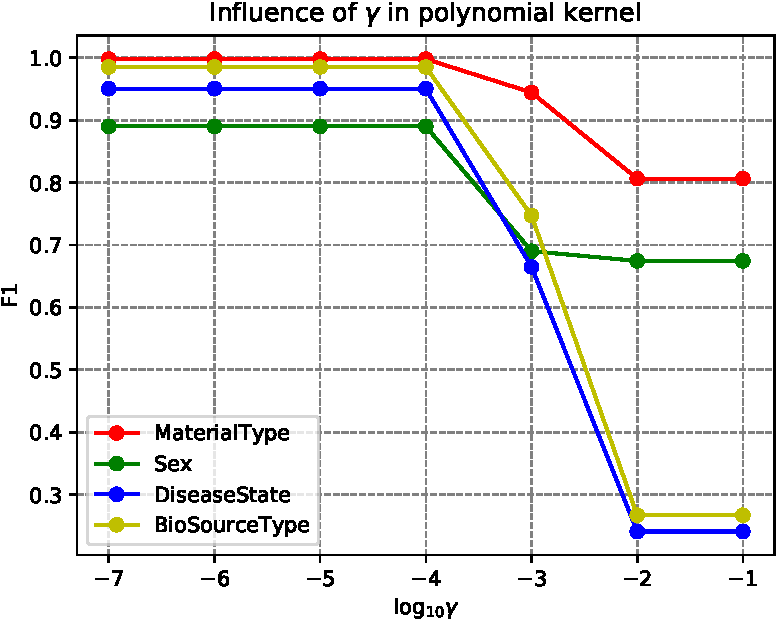
\includegraphics[width=0.8\linewidth]{../figs/gamma_poly}
\caption{Influence of $\gamma$ in polynomial kernel.}
\label{fig:gamma_poly}
\end{figure}

\begin{figure}[h]
\centering
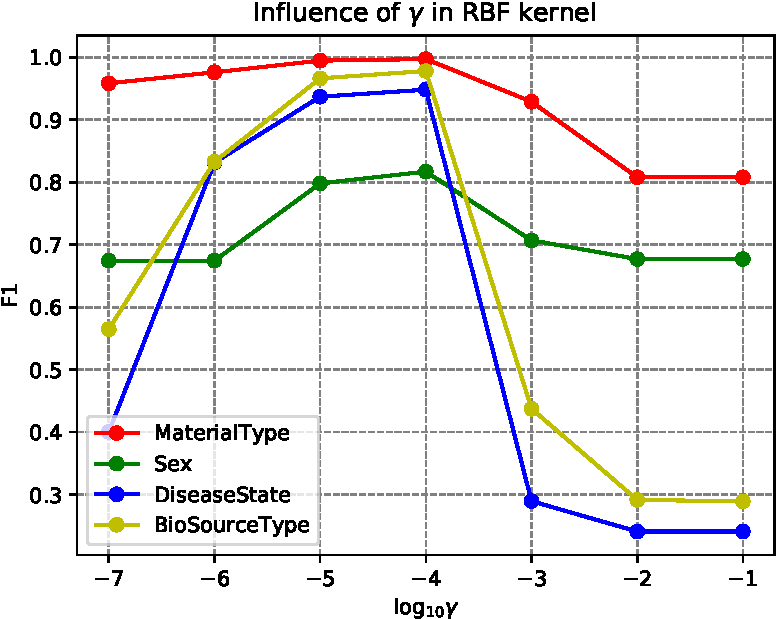
\includegraphics[width=0.8\linewidth]{../figs/gamma_rbf}
\caption{Influence of $\gamma$ in RBF kernel.}
\label{fig:gamma_rbf}
\end{figure}

\begin{figure}[h]
\centering
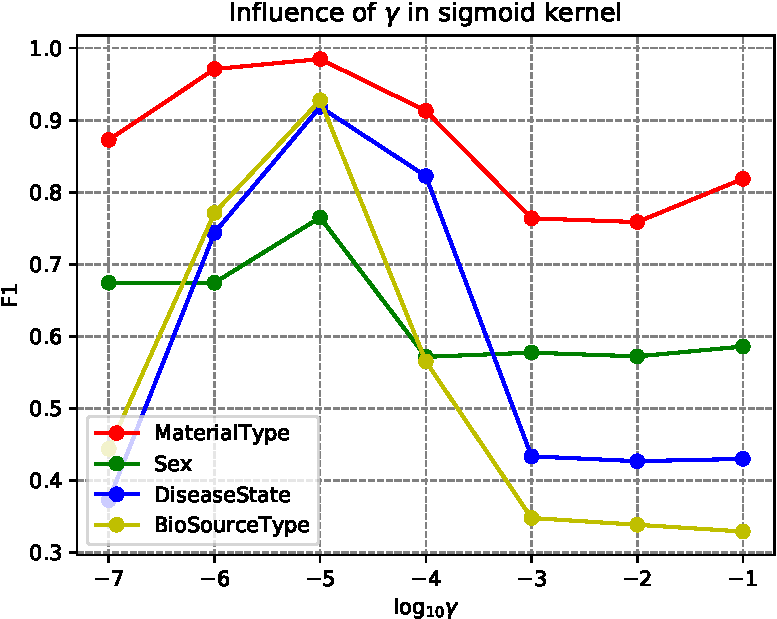
\includegraphics[width=0.8\linewidth]{../figs/gamma_sigmoid}
\caption{Influence of $\gamma$ in sigmoid kernel.}
\label{fig:gamma_sigmoid}
\end{figure}


We then set $\gamma$ as the best value and further evaluate the influence of $C$ in different kernels. the results are shown in Figure~\ref{fig:C_poly}, \ref{fig:C_rbf} and \ref{fig:C_sigmoid}. We can find that for all the 3 kernels and all the 4 tasks, when $C$ is heavily small, the performance is extremely poor. This is because when $C$ is very small, we allow many of the sample to be classified to the wrong class, which may hurt model's performance. As $C$ grows, the performance of both polymomial and RBF kernels grows consistently while the performance of sigmoid kernel has a small drop in the end. 


\begin{figure}[h]
\centering
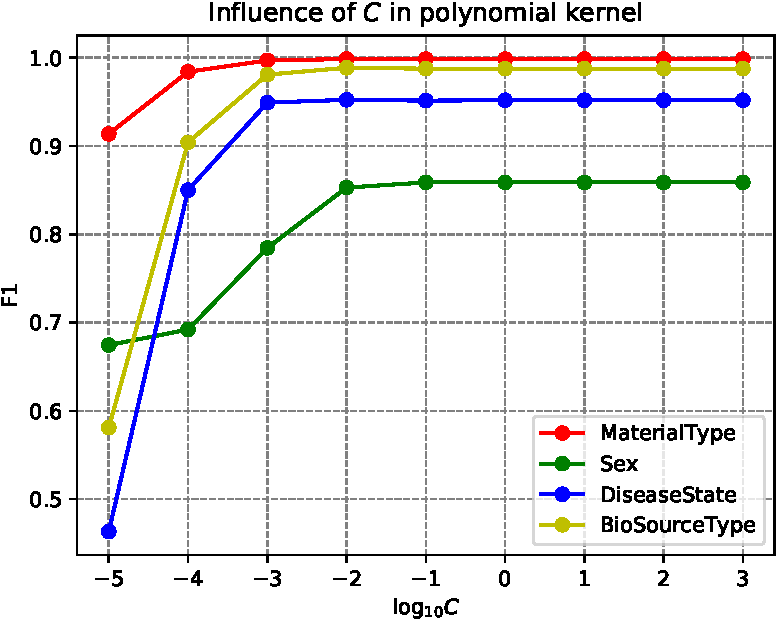
\includegraphics[width=0.8\linewidth]{../figs/C_poly}
\caption{Influence of $C$ in polynomial kernels}
\label{fig:C_poly}
\end{figure}

\begin{figure}[h]
\centering
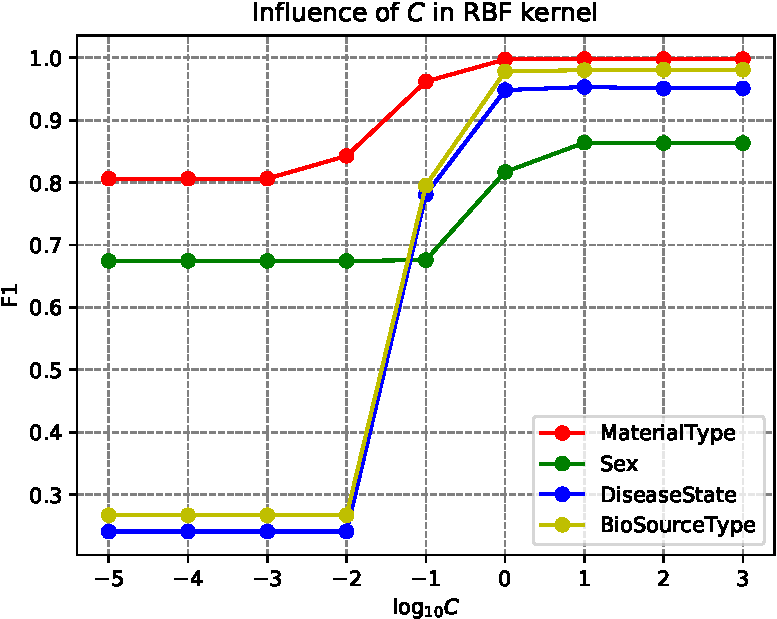
\includegraphics[width=0.8\linewidth]{../figs/C_rbf}
\caption{Influence of $C$ in RBF kernels}
\label{fig:C_rbf}
\end{figure}


\begin{figure}[h]
\centering
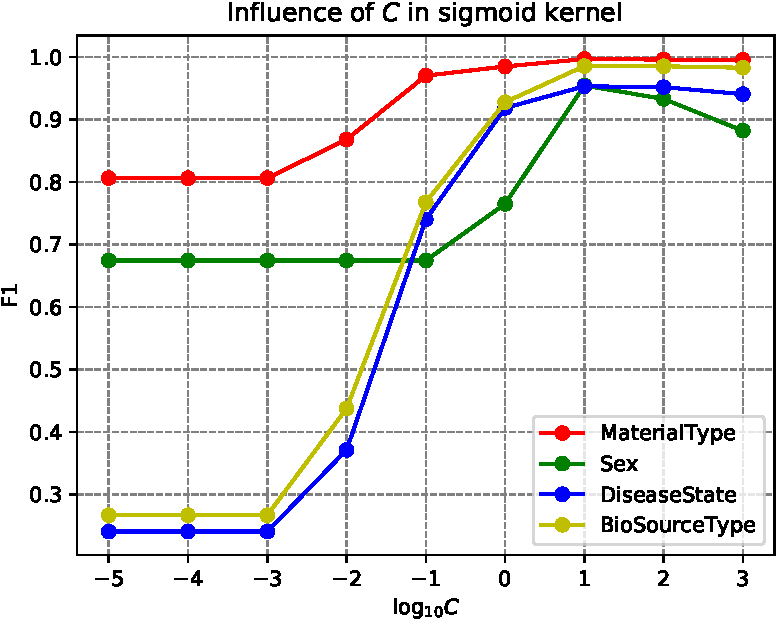
\includegraphics[width=0.8\linewidth]{../figs/C_sigmoid}
\caption{Influence of $C$ in sigmoid kernels}
\label{fig:C_sigmoid}
\end{figure}


After extensive experiments on SVM, we get the best parameter settings for the four tasks shown in Tabel~\ref{tab:SVM}.


	\begin{table}[tbp]
		\centering
		\begin{tabular}{l|cccc}
			\toprule
			{Label Type} & $F_1 (\%)$ & Kernel &$\gamma$ & $C$ \\
			\midrule
			{\textit{MaterialType}}&99.85 & polynomial &1e-3&1\\
			{\textit{Sex}}		& 95.44 & sigmoid    &1e-5&10 \\
			{\textit{DiseaseState}}& 95.31 & sigmoid &1e-5&10\\
			{\textit{BioSourceType}}& 98.76 & polynomial &1e-3&1\\
			\bottomrule	
		\end{tabular}
		\caption{Best parameter settings for SVM model. }
		\label{tab:SVM}
	\end{table}

	 
	\subsection{Random Forest}
	For random forest, we adjust many hyperparameters incluing: maximum feature number, maximum tree depth, minimal samples in split node and minimal samples in leaf node. Extensive experiments show that most of the hyperparameters have less or no influence on the results. We argue that this is because the data is quite linear separable, thus such ensemble methods can not leverage its best ability. 
	
	Only one hyper parameter have influence on the results, which is minimal samples in leaf node (\textit{min\_samples\_leaf}) and is shown in Figure~\ref{fig:min_samples_leaf}. We find that with the growing of \textit{min\_samples\_leaf}, the performance of all the 4 tasks decrease consistently. We think this is because random forest is a ensemble method and each weak classifier (decision tree here) should be somehow overfitted to the data (\textit{min\_samples\_leaf}), which enhance the whole model's diversity.
	
	The best results for 4 tasks are shown in Tabel~\ref{tab:RF}.
	\begin{table}[tbp]
		\centering
		\begin{tabular}{l|cc}
			\toprule
			{Label Type} & $F_1 (\%)$& \textit{min\_samples\_leaf}  \\
			\midrule
			{\textit{MaterialType}}&99.35 &1\\
			{\textit{Sex}}		& 80.14  &1\\
			{\textit{DiseaseState}}& 94.41&1 \\
			{\textit{BioSourceType}}& 97.20 &1\\
			\bottomrule	
		\end{tabular}
		\caption{Best parameter settings for random forest model. }
		\label{tab:RF}
	\end{table}
	 
	
\begin{figure}[h]
\centering
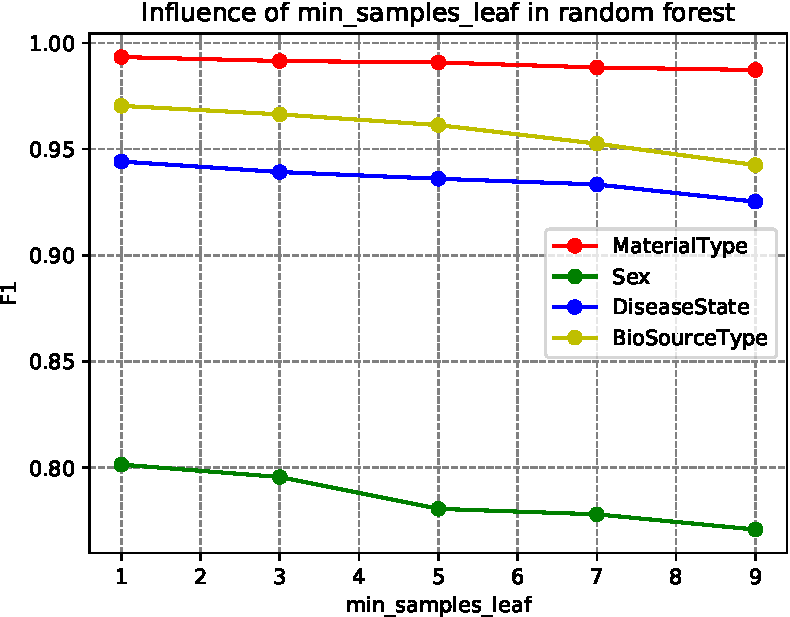
\includegraphics[width=0.8\linewidth]{../figs/min_samples_leaf}
\caption{Influence of \textit{min\_samples\_leaf} in random forest.}
\label{fig:min_samples_leaf}
\end{figure}
	

\subsection{Deep Forets}
Since the features do not have any locality or direct relationship, we only employ the cascade forest structure with 1 random forest (10 trees) and 1 completely-random tree forests (10 trees) in each level. As a extension to the original deep forest \cite{zhou2017deep}, we also add a LR model in each level to boost the performance of it. 

We find that when applied on 4 different tasks, the final levels of deep forest varies. The results are shown in Tabel~\ref{tab:DeepForest}. We can find that Deep forest beat random forest in all the 4 tasks, which indicates that such \textit{deep} variant of traditional works. We also noticed that the performance of deep forest is compatible to SVM, and we argue that this is because of the data's distribution.
\begin{table}[tbp]
	\centering
	\begin{tabular}{l|cc}
		\toprule
		{Label Type} & $F_1 (\%)$&Depth\\
		\midrule
		{\textit{MaterialType}}&99.83 &5\\
		{\textit{Sex}}		& 92.90  &9\\
		{\textit{DiseaseState}}& 95.58 &8 \\
		{\textit{BioSourceType}}& 98.62 &5\\
		\bottomrule	
	\end{tabular}
	\caption{Best parameter settings for random forest model. }
	\label{tab:DeepForest}
\end{table}

\subsection{Deep Neural Network}

\subsubsection{ NN on PCA-processed data}
At first we try deep neural network on   PCA-processed data. The dimension is 500, and the network is shown in Figure~\ref{nn_1}. Besides,  we use L2 regularization and dropout to avoid overfitting. The dropout rate is 0.50. In the end, we use batch normalization in each layer and it greatly improves the performance. The results and selected parameters are shown in Table~\ref{nnpca_result}.
	
	\begin{table}[tbp]
		\centering
		\begin{tabular}{l|cccc}
			\toprule
			{Label Type} & $F_1 (\%)$ & learning rate &$batch size$  \\
			\midrule
			{\textit{MaterialType}}&99.30 & 0.001 &32\\
			{\textit{Sex}}		& 92.92 & 0.001    &50 \\
			{\textit{DiseaseState}}& 94.38 & 0.001 &32\\
			{\textit{BioSourceType}}& 95.87 & 0.001 &16\\
			\bottomrule	
		\end{tabular}
		
		\caption{Best results and parameter settings for NN model on PCA data. }
		\label{nnpca_result}
	\end{table}
	
	Besides, we visualize the training process of Sex and Bio tasks with the change of learning. It is shown in Figure~\ref{lr_result}, and it can be seen $lr=0.001$ is the best result in four task. 
	
	\begin{figure}[]
		\centering
		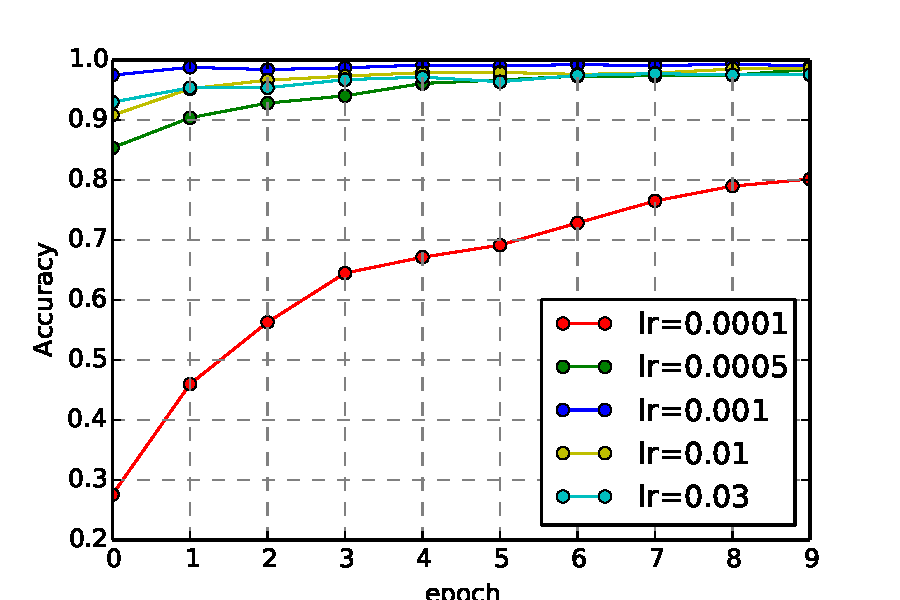
\includegraphics[width=0.2\textwidth]{../figs/lr_acc_bio.pdf}
		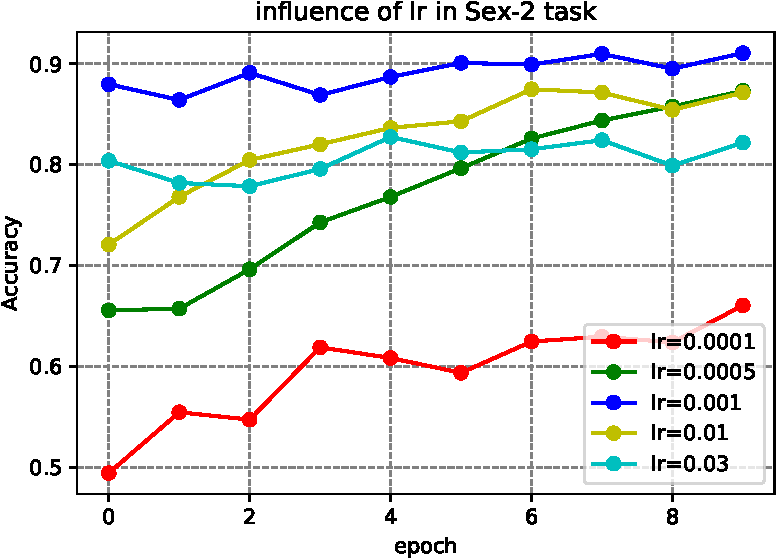
\includegraphics[width=0.2\textwidth]{../figs/lr_acc_sex.pdf}
		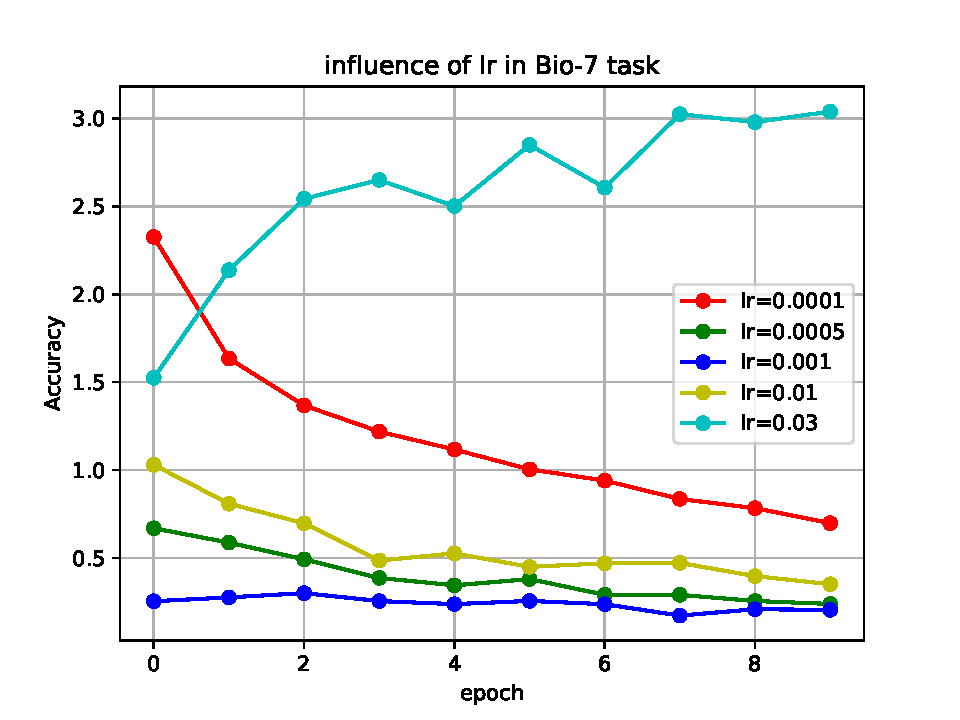
\includegraphics[width=0.2\textwidth]{../figs/lr_loss_bio.pdf}
		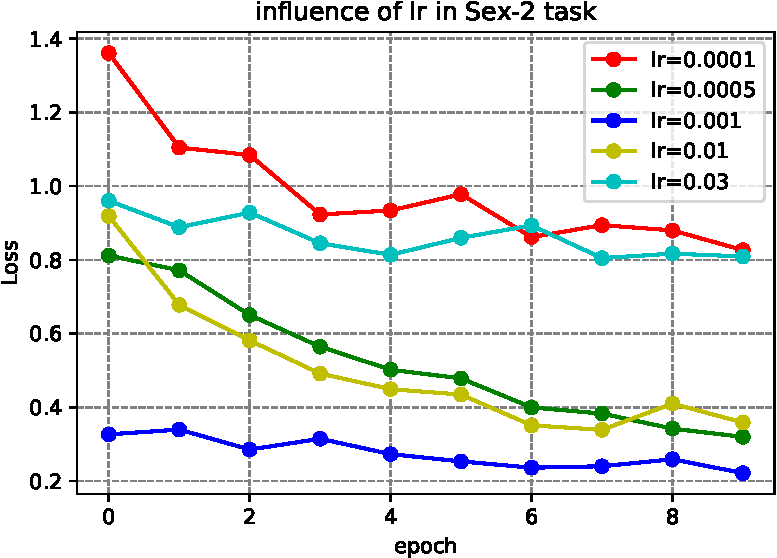
\includegraphics[width=0.2\textwidth]{../figs/lr_loss_sex.pdf}
		\caption{a.accuracy in Bio task;  b, accuracy in Sex task; c, loss in Bio task; d, loss in Sex task (From left to right and top to down). }
		\label{lr_result}
		\centering
	\end{figure}
	
	
	\subsubsection{ NN on raw data}
	To improve the NN' performance, we try deep neural network on  raw data. Because it is a nonlinear classifier, it may solve the relevant of raw data feature by itself. The dimension is 22283, and the network is shown in Figure~\ref{nn_1}. The setting of L2 regularization, dropout and batch normalization is same as the above experiment. But without the proper initialization (e.g. random initialization), the performance is not better than NN above. On the contrary, the accuracy is only at around 70\%, for it is easily influenced by local optimization. So we use greedy layer-wise pre training method to initialize the weights using 3 different neural network (which have the same structure as autoencoder) . Then the performance is improved a lot, besides the train process becoming faster. The best result and seleted parameters is shown in Table~{\ref{nnraw_result}.\\
			
			\begin{table}[tbp]
				\centering
				\begin{tabular}{l|cccc}
					\toprule
					{Label Type} & $F_1 (\%)$ & learning rate &$batch size$  \\
					\midrule
					{\textit{MaterialType}}&99.78 & 0.001 &32\\
					{\textit{Sex}}		& 92.41 & 0.01    &50 \\
					{\textit{DiseaseState}}& 94.37 & 0.001 &32\\
					{\textit{BioSourceType}}& 98.35 & 0.001 &32\\
					\bottomrule	
				\end{tabular}
				
				\caption{Best results and parameter settings for NN model on raw data. }
				\label{nnraw_result}
			\end{table}
			
			Compared with Table~\ref{nnpca_result}, it can be seen that MaterialType task and BioSourceType task has been improved, but the Sex task and DiseaseState task did not become higher. Besides, there are some differences among the optimal parameters. 




	\begin{acks}
	This work is successfully produced thanks to the kind guidance from and discussion with Prof. Bo Yuan.
	\end{acks}
	
	
	
	{\small
		\bibliographystyle{ACM-Reference-Format}
		\bibliography{bibliography} 	
	}
	

\end{document}